\documentclass[12pt]{article}
\usepackage{amsmath, amssymb}
\usepackage{geometry}
\geometry{margin=1in}
\usepackage{tikz}
\usetikzlibrary{decorations.pathreplacing, arrows.meta}

\title{Analytical Solution of the Viscous Burgers’ Equation\\ via the Cole–Hopf Transformation}
\author{}
\date{}

\begin{document}
\maketitle
Objective:
The primary goal of this study is to generate a high-fidelity classical solution to this problem using:
An analytical solution via the Cole-Hopf transformation,which will serve as a benchmark for evaluating the accuracy and efficiency of emerging quantum-enhanced PDE solvers, such as the Quantum Tensor Network (QTN) and Hydrodynamic Schrödinger Equation (HSE) frameworks.
\vspace{2mm}

Our main focus would be Sod problem, also known as the Sod's shock tube problem, is a classic one-dimensional Riemann problem used to test the accuracy of computational fluid dynamics (CFD) codes. It involves a shock tube initially divided into two regions with different pressures and densities. At time t=0, the division is removed, and the resulting wave interactions (shock wave, rarefaction wave, and contact discontinuity) are analyzed. 

\vspace{3mm}

 Key Features of the Sod Problem:
Exact Solution:
The Sod problem has an analytical solution (or an exact solution) which is used as a reference to validate numerical solutions from CFD codes.
Discontinuities:
The problem contains discontinuities (shock waves and contact discontinuities) which are challenging to simulate accurately with numerical methods.



\section*{1. Problem Statement}

We consider a one-dimensional sod shock tube of length L, initially partitioned into two regions by an imaginary membrane. The tube contains a scalar compressible fluid velocity field u(x,t), governed by the viscous Burgers equation:
\begin{equation}
\frac{\partial u}{\partial t} + u \frac{\partial u}{\partial x} = \nu \frac{\partial^2 u}{\partial x^2}
\end{equation} 
\vspace{5mm}


\begin{center}
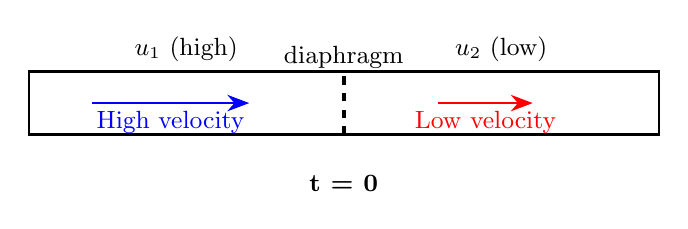
\begin{tikzpicture}[scale=0.8, every node/.style={font=\small}]

  \draw[thick] (0,0) rectangle (10,1);

  \draw[ultra thick, dashed] (5,0) -- (5,1) node[midway, above=3mm] {diaphragm};
  

  \node[above] at (2.5,1) {$u_1$ (high)};
  \node[above] at (7.5,1) {$u_2$ (low)};
  
 
  \draw[-{Stealth[scale=1.2]}, thick, blue] (1,0.5) -- (3.5,0.5);
  \draw[-{Stealth[scale=1.2]}, thick, red] (6.5,0.5) -- (8,0.5);
  \node[blue] at (2.25,0.2) {High velocity};
  \node[red] at (7.25,0.2) {Low velocity};
  
  
  \node[below] at (5,-0.5) {\textbf{t = 0}};
\end{tikzpicture}
\end{center}

\vspace{5mm}


\begin{center}
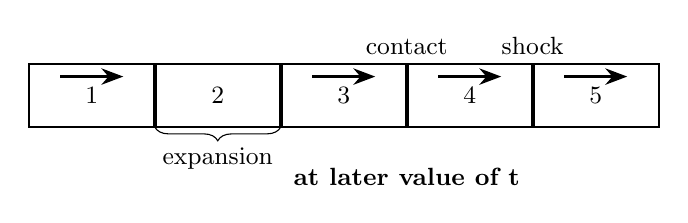
\begin{tikzpicture}[scale=0.8, every node/.style={font=\small}]
  % Tube
  \draw[thick] (0,0) rectangle (10,1);
  

  \draw[ultra thick] (2,0) -- (2,1);  % Expansion left
  \draw[ultra thick] (4,0) -- (4,1);  % Expansion right
  \draw[ultra thick] (6,0) -- (6,1);  % Contact
  \draw[ultra thick] (8,0) -- (8,1);  % Shock
  
  
  \node at (1,0.5) {1};
  \node at (3,0.5) {2};
  \node at (5,0.5) {3};
  \node at (7,0.5) {4};
  \node at (9,0.5) {5};
  

  \draw [decorate, decoration={brace, amplitude=5pt, mirror}] (2,0) -- (4,0) 
      node [midway, below=4pt] {expansion};
  \node[above] at (6,1) {contact};
  \node[above] at (8,1) {shock};
  
 
  \draw[-{Stealth[scale=1.2]}, thick] (0.5,0.8) -- (1.5,0.8);
  \draw[-{Stealth[scale=1.2]}, thick] (4.5,0.8) -- (5.5,0.8);
  \draw[-{Stealth[scale=1.2]}, thick] (6.5,0.8) -- (7.5,0.8);
  \draw[-{Stealth[scale=1.2]}, thick] (8.5,0.8) -- (9.5,0.8);
  
  \node[below] at (6,-0.5) {\textbf{at later value of t}};
\end{tikzpicture}
\end{center}

for $x \in [0,1]$ and $t > 0$, where $u(x, t)$ is the velocity field and $\nu > 0$ is the viscosity.


\textbf{Initial condition:}
\[
u(x, 0) =
\begin{cases}
1, & x \leq 0.5 \\
0, & x > 0.5
\end{cases}
\]

\textbf{Boundary conditions:}
\[
u(0, t) = 1, \qquad u(1, t) = 0 \qquad \forall\, t > 0
\]
 Wave Phenomena:
When the diaphragm is removed, the pressure difference drives the fluid. This creates a shock wave that propagates into the lower-pressure region, and a rarefaction wave that propagates into the higher-pressure region.
A contact discontinuity also forms between the two regions, separating the two fluids.  



The contact discontinuity is a region where density and entropy can change, but pressure and the normal component of velocity are constant across it. 




\section*{2. Linearization via Cole--Hopf Transformation}

Introduce the Cole--Hopf transformation:
\begin{equation}
u(x, t) = -2\nu \frac{\frac{\partial}{\partial x} \varphi(x, t)}{\varphi(x, t)}
\quad \text{or} \quad
u(x, t) = -2\nu \frac{\varphi_x(x, t)}{\varphi(x, t)}
\end{equation}
where $\varphi(x, t)$ is a new function to be determined.

\textit{Purpose:} This transformation converts the nonlinear Burgers' equation into a linear partial differential equation for $\varphi(x, t)$.

\section*{3. Derivation and Simplification of the Heat Equation}

\textbf{Time derivative of $u(x, t)$:}
\begin{align*}
\frac{\partial u}{\partial t}
&= -2\nu \frac{\partial}{\partial t} \left( \frac{\varphi_x}{\varphi} \right )
= -2\nu \left( \frac{\varphi_{xt}}{\varphi} - \frac{\varphi_x \varphi_t}{\varphi^2} \right )
\end{align*}

\textbf{Spatial derivatives:}
\begin{align*}
\frac{\partial u}{\partial x}
&= -2\nu \frac{\partial}{\partial x} \left( \frac{\varphi_x}{\varphi} \right )
= -2\nu \left( \frac{\varphi_{xx}}{\varphi} - \frac{\varphi_x^2}{\varphi^2} \right ) \\
u \frac{\partial u}{\partial x}
&= \left(-2\nu \frac{\varphi_x}{\varphi}\right) \left(-2\nu \left( \frac{\varphi_{xx}}{\varphi} - \frac{\varphi_x^2}{\varphi^2}\right)\right) \\
&= 4\nu^2 \frac{\varphi_x}{\varphi} \left( \frac{\varphi_{xx}}{\varphi} - \frac{\varphi_x^2}{\varphi^2} \right )
\end{align*}
\[
\frac{\partial^2 u}{\partial x^2}
= -2\nu \frac{\partial}{\partial x} \left( \frac{\varphi_{xx}}{\varphi} - \frac{\varphi_x^2}{\varphi^2} \right )
\]

\textbf{Substitute into the original equation and simplify:}

Equation reduces to:
\[
\boxed{
\frac{\partial \varphi}{\partial t} = \nu \frac{\partial^2 \varphi}{\partial x^2}
}
\]
which is the classical heat (diffusion) equation for $\varphi(x, t)$.

\section*{4. Setup of Initial and Boundary Conditions for $\varphi$}

\subsection*{(a) Initial Condition}

From the Cole--Hopf formula at $t = 0$:
\[
u(x,0) = -2\nu \frac{\varphi_x(x,0)}{\varphi(x,0)}
\implies \frac{\varphi_x(x,0)}{\varphi(x,0)} = -\frac{u(x,0)}{2\nu}
\]
Integrate both sides from $0$ to $x$:
\[
\ln \varphi(x,0) = -\frac{1}{2\nu} \int_0^x u(s,0)\,ds + C
\]
Therefore,
\[
\varphi(x, 0) = A\, \exp\left( -\frac{1}{2\nu} \int_0^x u(s, 0)\, ds \right )
\]
where $A = e^C$ is an irrelevant constant.

For the given step initial condition:
\[
\int_0^x u(s, 0)\, ds =
\begin{cases}
x & (x \le 0.5) \\
0.5 & (x > 0.5)
\end{cases}
\]
So,
\[
\boxed{
\varphi(x, 0) =
\begin{cases}
e^{-x/(2\nu)}, & x \leq 0.5 \\
e^{-0.5/(2\nu)}, & x > 0.5
\end{cases}
}
\]

\subsection*{(b) Boundary Conditions}

Using the Cole--Hopf relation at the boundaries:
\[
u(x, t) = -2\nu \frac{\varphi_x(x, t)}{\varphi(x, t)}
\]
At $x = 0$:
\[
u(0, t) = 1 \implies -2\nu \frac{\varphi_x(0, t)}{\varphi(0, t)} = 1 
\implies \varphi_x(0, t) = -\frac{1}{2\nu} \varphi(0, t)
\]
At $x = 1$:
\[
u(1, t) = 0 \implies \varphi_x(1, t) = 0
\]
So,
\[
\boxed{
\begin{aligned}
\varphi_x(0, t) &= -\frac{1}{2\nu} \varphi(0, t) \\
\varphi_x(1, t) &= 0
\end{aligned}
}
\]

\section*{5. Solution to the Heat Equation}

We solve
\[
\frac{\partial \varphi}{\partial t} = \nu \frac{\partial^2 \varphi}{\partial x^2}
\]
with initial and boundary conditions as above.

\subsection*{Analytical Solution on Infinite or Simple Domains (for reference)}
With homogeneous Dirichlet or Neumann boundaries, the heat equation is classically solved using Fourier series or with the heat kernel:
\[
\varphi(x, t) = \int_{-\infty}^{\infty}
    \frac{1}{\sqrt{4\pi \nu t}}
    \exp\left( -\frac{(x-y)^2}{4\nu t} \right)
    \varphi(y, 0)\,dy
\]
This form gives the exact solution for infinite or periodic domains.

\subsection*{Solution with (Mixed) Boundary Conditions in this Problem}
For the mixed (Robin/Neumann) boundary conditions in this problem:
\[
\varphi_x(0, t) = -\frac{1}{2\nu} \varphi(0, t),\qquad \varphi_x(1, t) = 0
\]
there is in general no closed-form analytical expression for all times. 

\textbf{Standard approach:} Solve the heat equation numerically using finite-difference methods. Discretize $x$ and $t$, and advance the solution $\varphi(x, t)$ forward, enforcing boundary conditions at each step.

\begin{itemize}
    \item Discretize the spatial domain: $x_i = i \Delta x,~i=0,\dots,N$
    \item At $x=0$: Apply $ \displaystyle \frac{\varphi_1^n - \varphi_0^n}{\Delta x} = -\frac{1}{2\nu} \varphi_0^n $
    \item At $x=1$: Apply $ \displaystyle \frac{\varphi_N^n - \varphi_{N-1}^n}{\Delta x} = 0 \implies \varphi_N^n = \varphi_{N-1}^n $
    \item Evolve using an explicit or implicit time-stepping scheme.
\end{itemize}

\section*{6. Recovery of the Burgers Solution}

Once $\varphi(x, t)$ is known (from numerical computation or explicit formula, where possible), recover $u(x, t)$ using:
\[
\boxed{
u(x, t) = -2\nu\, \frac{\frac{\partial}{\partial x} \varphi(x, t)}{\varphi(x, t)}
}
\]

\textbf{In practice:}
\[
\left. \frac{\partial}{\partial x} \varphi(x, t) \right|_{x_i} \approx \frac{\varphi(x_{i+1}, t) - \varphi(x_{i-1}, t)}{2\Delta x}
\]
Evaluate at every internal grid point, then used the formula above.

\section*{7. Final Summary Table}

\begin{center}
\renewcommand{\arraystretch}{1.25}
\begin{tabular}{|l|l|l|}
\hline
\textbf{Step} & \textbf{Description} & \textbf{Mathematical Formulation} \\
\hline
1 & Cole--Hopf transformation & $u = -2\nu\, \dfrac{\varphi_x}{\varphi}$ \\
2 & Heat equation for $\varphi$ & $\,\dfrac{\partial \varphi}{\partial t} = \nu \dfrac{\partial^2 \varphi}{\partial x^2}$ \\
3 & Initial condition & $\varphi(x,0) = \begin{cases} e^{-x/(2\nu)}, & x \leq 0.5 \\ e^{-0.5/(2\nu)}, & x > 0.5 \end{cases}$ \\
4 & Boundary conditions & $\varphi_x(0, t) = -\dfrac{1}{2\nu} \varphi(0, t),~\varphi_x(1, t) = 0$ \\
5 & Solve for $\varphi$ & Numerical solution for $\varphi(x, t)$ with above data \\
6 & Recover $u(x, t)$ & $u(x, t) = -2\nu \dfrac{\varphi_x(x, t)}{\varphi(x, t)}$ \\
\hline
\end{tabular}
\end{center}


\section*{Summary}

Each step---from nonlinear PDE to linear problem, careful setup of initial and boundary data, followed by solution and recovery of the physical answer---has been rigorously established and is standard in applied mathematics and partial differential equations.

\end{document}

